% Maschenstromverfahren nach Brinkmeyer Aufg. 27
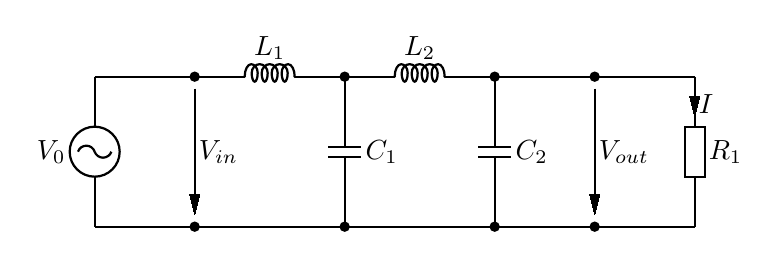
\begin{tikzpicture}[scale=2.54]%
% dpic version 2024.01.01 option -g for TikZ and PGF 1.01
\ifx\dpiclw\undefined\newdimen\dpiclw\fi
\global\def\dpicdraw{\draw[line width=\dpiclw]}
\global\def\dpicstop{;}
\dpiclw=0.8bp
\dpiclw=0.8bp
\dpicdraw (0,0)
 --(0,-0.25)\dpicstop
\dpicdraw (0,-0.375) circle (0.049213in)\dpicstop
\dpicdraw (-0,-0.375)
 ..controls (-0.005978,-0.357065) and (-0.022762,-0.344968)
 ..(-0.041667,-0.344968)
 ..controls (-0.060571,-0.344968) and (-0.077355,-0.357065)
 ..(-0.083333,-0.375)\dpicstop
\dpicdraw (0,-0.375)
 ..controls (0.005978,-0.392935) and (0.022762,-0.405032)
 ..(0.041667,-0.405032)
 ..controls (0.060571,-0.405032) and (0.077355,-0.392935)
 ..(0.083333,-0.375)\dpicstop
\dpicdraw (0,-0.5)
 --(0,-0.75)\dpicstop
\draw (-0.125,-0.375) node[left=-2bp]{$ V_0$};
\dpicdraw (0,0)
 --(0.5,0)\dpicstop
\dpicdraw[fill=black](0.5,0) circle (0.007874in)\dpicstop
\dpicdraw[fill=black](0.5,-0.75) circle (0.007874in)\dpicstop
\filldraw[line width=0bp](0.475,-0.59)
 --(0.5,-0.69)
 --(0.525,-0.59) --cycle\dpicstop
\dpicdraw (0.5,-0.06)
 --(0.5,-0.667094)\dpicstop
\draw (0.5,-0.375) node[right=-2bp]{$ V_{in}$};
\dpicdraw (0.5,0)
 --(0.75,0)\dpicstop
\dpicdraw[line width=0.4bp](0.75,0) circle (0.00109in)\dpicstop
\dpicdraw (0.75,0)
 ..controls (0.75,0.034375) and (0.764625,0.0625)
 ..(0.7825,0.0625)
 ..controls (0.800375,0.0625) and (0.815,0.042813)
 ..(0.815,0.01875)
 ..controls (0.815,-0.005313) and (0.80825,-0.025)
 ..(0.8,-0.025)
 ..controls (0.79175,-0.025) and (0.785,-0.005313)
 ..(0.785,0.01875)
 ..controls (0.785,0.042813) and (0.803,0.0625)
 ..(0.825,0.0625)
 ..controls (0.847,0.0625) and (0.865,0.042813)
 ..(0.865,0.01875)
 ..controls (0.865,-0.005313) and (0.85825,-0.025)
 ..(0.85,-0.025)
 ..controls (0.84175,-0.025) and (0.835,-0.005313)
 ..(0.835,0.01875)
 ..controls (0.835,0.042813) and (0.853,0.0625)
 ..(0.875,0.0625)
 ..controls (0.897,0.0625) and (0.915,0.042813)
 ..(0.915,0.01875)
 ..controls (0.915,-0.005313) and (0.90825,-0.025)
 ..(0.9,-0.025)
 ..controls (0.89175,-0.025) and (0.885,-0.005313)
 ..(0.885,0.01875)
 ..controls (0.885,0.042813) and (0.903,0.0625)
 ..(0.925,0.0625)
 ..controls (0.947,0.0625) and (0.965,0.042813)
 ..(0.965,0.01875)
 ..controls (0.965,-0.005313) and (0.95825,-0.025)
 ..(0.95,-0.025)
 ..controls (0.94175,-0.025) and (0.935,-0.005313)
 ..(0.935,0.01875)
 ..controls (0.935,0.042813) and (0.949625,0.0625)
 ..(0.9675,0.0625)
 ..controls (0.985375,0.0625) and (1,0.034375)
 ..(1,0)\dpicstop
\dpicdraw[line width=0.4bp](1,0) circle (0.00109in)\dpicstop
\dpicdraw (1,0)
 --(1.25,0)\dpicstop
\draw (0.875,0.0625) node[above=-2bp]{$ L_1$};
\dpicdraw[fill=black](1.25,0) circle (0.007874in)\dpicstop
\dpicdraw (1.25,0)
 --(1.25,-0.35)\dpicstop
\dpicdraw (1.166667,-0.35)
 --(1.333333,-0.35)\dpicstop
\dpicdraw (1.166667,-0.4)
 --(1.333333,-0.4)\dpicstop
\dpicdraw (1.25,-0.4)
 --(1.25,-0.75)\dpicstop
\draw (1.333333,-0.375) node[right=-2bp]{$ C_1$};
\dpicdraw[fill=black](1.25,-0.75) circle (0.007874in)\dpicstop
\dpicdraw (1.25,0)
 --(1.5,0)\dpicstop
\dpicdraw[line width=0.4bp](1.5,0) circle (0.00109in)\dpicstop
\dpicdraw (1.5,0)
 ..controls (1.5,0.034375) and (1.514625,0.0625)
 ..(1.5325,0.0625)
 ..controls (1.550375,0.0625) and (1.565,0.042813)
 ..(1.565,0.01875)
 ..controls (1.565,-0.005313) and (1.55825,-0.025)
 ..(1.55,-0.025)
 ..controls (1.54175,-0.025) and (1.535,-0.005313)
 ..(1.535,0.01875)
 ..controls (1.535,0.042813) and (1.553,0.0625)
 ..(1.575,0.0625)
 ..controls (1.597,0.0625) and (1.615,0.042813)
 ..(1.615,0.01875)
 ..controls (1.615,-0.005313) and (1.60825,-0.025)
 ..(1.6,-0.025)
 ..controls (1.59175,-0.025) and (1.585,-0.005313)
 ..(1.585,0.01875)
 ..controls (1.585,0.042813) and (1.603,0.0625)
 ..(1.625,0.0625)
 ..controls (1.647,0.0625) and (1.665,0.042813)
 ..(1.665,0.01875)
 ..controls (1.665,-0.005313) and (1.65825,-0.025)
 ..(1.65,-0.025)
 ..controls (1.64175,-0.025) and (1.635,-0.005313)
 ..(1.635,0.01875)
 ..controls (1.635,0.042813) and (1.653,0.0625)
 ..(1.675,0.0625)
 ..controls (1.697,0.0625) and (1.715,0.042813)
 ..(1.715,0.01875)
 ..controls (1.715,-0.005313) and (1.70825,-0.025)
 ..(1.7,-0.025)
 ..controls (1.69175,-0.025) and (1.685,-0.005313)
 ..(1.685,0.01875)
 ..controls (1.685,0.042813) and (1.699625,0.0625)
 ..(1.7175,0.0625)
 ..controls (1.735375,0.0625) and (1.75,0.034375)
 ..(1.75,0)\dpicstop
\dpicdraw[line width=0.4bp](1.75,0) circle (0.00109in)\dpicstop
\dpicdraw (1.75,0)
 --(2,0)\dpicstop
\draw (1.625,0.0625) node[above=-2bp]{$ L_2$};
\dpicdraw[fill=black](2,0) circle (0.007874in)\dpicstop
\dpicdraw (2,0)
 --(2,-0.35)\dpicstop
\dpicdraw (1.916667,-0.35)
 --(2.083333,-0.35)\dpicstop
\dpicdraw (1.916667,-0.4)
 --(2.083333,-0.4)\dpicstop
\dpicdraw (2,-0.4)
 --(2,-0.75)\dpicstop
\draw (2.083333,-0.375) node[right=-2bp]{$ C_2$};
\dpicdraw[fill=black](2,-0.75) circle (0.007874in)\dpicstop
\dpicdraw (2,0)
 --(2.5,0)\dpicstop
\dpicdraw[fill=black](2.5,0) circle (0.007874in)\dpicstop
\dpicdraw[fill=black](2.5,-0.75) circle (0.007874in)\dpicstop
\filldraw[line width=0bp](2.475,-0.59)
 --(2.5,-0.69)
 --(2.525,-0.59) --cycle\dpicstop
\dpicdraw (2.5,-0.06)
 --(2.5,-0.667094)\dpicstop
\draw (2.5,-0.375) node[right=-2bp]{$ V_{out}$};
\dpicdraw (2.5,0)
 --(3,0)\dpicstop
\dpicdraw (3,0)
 --(3,-0.25)\dpicstop
\dpicdraw (3,-0.5)
 --(3.05,-0.5)
 --(3.05,-0.25)
 --(2.95,-0.25)
 --(2.95,-0.5)
 --(3,-0.5)\dpicstop
\dpicdraw (3,-0.5)
 --(3,-0.75)\dpicstop
\draw (3.05,-0.375) node[right=-2bp]{$ R_1$};
\filldraw[line width=0bp](2.975,-0.1)
 --(3,-0.2)
 --(3.025,-0.1) --cycle\dpicstop
\dpicdraw (3,-0.177094)
 --(3,-0.1)\dpicstop
\draw (3,-0.138547) node[right=-2bp]{$ I$};
\dpicdraw (3,-0.75)
 --(0,-0.75)\dpicstop
\end{tikzpicture}%
